%% Template article for Elsevier's document class `elsarticle'
%% with numbered style bibliographic references
\documentclass[preprint,12pt]{elsarticle}

% remove preprint footnote
\makeatletter
\def\ps@pprintTitle{%
 \let\@oddhead\@empty
 \let\@evenhead\@empty
 \def\@oddfoot{\centerline{\thepage}}%
 \let\@evenfoot\@oddfoot}
\makeatother


\usepackage{setspace}
\doublespacing

\usepackage{hyperref} % auto detect ref type
\usepackage{natbib}
\setcitestyle{authoryear}

%% Use the option review to obtain double line spacing
%% \documentclass[preprint,review,12pt]{elsarticle}

%% Use the options 1p,twocolumn; 3p; 3p,twocolumn; 5p; or 5p,twocolumn
%% for a journal layout:
%% \documentclass[final,1p,times]{elsarticle}
%% \documentclass[final,1p,times,twocolumn]{elsarticle}
%% \documentclass[final,3p,times]{elsarticle}
%% \documentclass[final,3p,times,twocolumn]{elsarticle}
%% \documentclass[final,5p,times]{elsarticle}
%% \documentclass[final,5p,times,twocolumn]{elsarticle}

\usepackage{graphicx}
\usepackage{amssymb}
\usepackage{amsmath}
\usepackage{caption}
\usepackage{textcomp}    % for Hawaii characters
%\usepackage{listings}
%\lstset{language=R}
\usepackage[T1]{fontenc}  % tilde in middle in lstlisting
\usepackage[formats]{listings}
\lstset{language=R,
		basicstyle=\ttfamily,
		columns=fixed,
		basewidth=0.5em,
		literate={~}{{$\sim$}}1
		}

\biboptions{comma,round}

% shortcuts
\newcommand{\bbeta}{\boldsymbol{\beta}}
\newcommand{\blambda}{\boldsymbol{\lambda}}
\newcommand{\T}{\intercal}
\newcommand{\bS}{\mathbf{S}}
\newcommand{\bQ}{\mathbf{Q}}
\newcommand{\bSigma}{\boldsymbol{\Sigma}}
\newcommand{\bm}{\boldsymbol}  % bold maths symbols
\newcommand{\tl}{\tilde{\lambda}}   % thinned little lambda
\newcommand{\tL}{\tilde{\Lambda}}  % thinned big lambda

% RJC 09/08/2019 Added shortcuts for Hawaiian words
\newcommand{\akepa}{\textquotesingle\={a}kepa}  % adds Hawaiian diacritical marks
\newcommand{\Akepa}{\textquotesingle\={A}kepa}  % adds Hawaiian diacritical marks
\newcommand{\hawaii}{Hawai\textquotesingle i}   % adds Hawaiian diacritical marks
\DeclareMathOperator*{\argmax}{arg\,max}  % * means _ puts thing beneath operator

\begin{document}
\begin{frontmatter}
\title{One-stage point transect distance sampling using iterated integrated nested Laplace approximations}

%% use the tnoteref command within \title for footnotes;
%% use the tnotetext command for the associated footnote;
%% use the fnref command within \author or \address for footnotes;
%% use the fntext command for the associated footnote;
%% use the corref command within \author for corresponding author footnotes;
%% use the cortext command for the associated footnote;
%% use the ead command for the email address,
%% and the form \ead[url] for the home page:
%%
%% \title{Title\tnoteref{label1}}
%% \tnotetext[label1]{}
%% \author{Name\corref{cor1}\fnref{label2}}
%% \ead{email address}
%% \ead[url]{home page}
%% \fntext[label2]{}
%% \cortext[cor1]{}
%% \address{Address\fnref{label3}}
%% \fntext[label3]{}


%% use optional labels to link authors explicitly to addresses:
%% \author[label1,label2]{<author name>}
%% \address[label1]{<address>}
%% \address[label,2]{<address>}

% RJC 09/08/2019 Added co-authors and affiliations. Note that I used \affil[]{} instead of \address[]{}
\author[1,*]{Andrew E Seaton}
\author[1,2]{Richard J Camp}
\author[3]{Finn Lindgren}
\author[1]{Janine B Illian}
\author[1]{David L Borchers}
\author[1]{David L Miller}      % Ask about co-authoring the manuscript
\author[1]{Len Thomas}          % Ask about co-authoring the manuscript
\author[1]{Stephen T Buckland}  % Ask about co-authoring the manuscript
\author[4]{Steve J Kendall}     % It is Steve's data we are using and I have already mentioned this manuscript to him.

%\address{Centre for Research into Ecological \& Environmental Modelling and School of Mathematics \& Statistics, University of St Andrews, St Andrews, Fife, Scotland}
\address[1]{Centre for Research into Ecological \& Environmental Modelling and School of Mathematics \& Statistics, University of St Andrews, St Andrews, Fife, Scotland}
\address[2]{U. S. Geological Survey, Pacific Island Ecosystems Research Center, P.O. Box 44, \hawaii{} National Park, HI 96718, U.S.A.}
\address[3]{School of Mathematics, University of Edinburgh, Edinburgh, Scotland}
\address[4]{U. S. Fish and Wildlife, Big Island National Wildlife Refuge Complex, 60 Nowelo St., Suite 100, Hilo, HI  96720, U.S.A.}
\address[*]{Correspondence: Andrew E Seaton, Email: aes22@st-andrews.ac.uk}

\begin{abstract}
Distance sampling methods aim to estimate the size and distribution of animal populations.  Traditionally this has been achieved using a two-stage approach by using first-stage estimates of detectability as an offset in a second-stage generalised additive model.  One-stage approaches have typically been implemented using MCMC and data augmentation methods. Here we present a new approach to one-stage distance sampling models, using iterated fits of latent Gaussian models fitted using integrated nested Laplace approximations (INLA) to simultaneously estimate the detectability and spatial distribution.  We model the data as a thinned log-Gaussian Cox process using computationally efficient Gaussian Markov random field approximations to Gaussian random fields.  We demonstrate the approach by applying the methods to point count survey data of Hawaiian \akepa{}. Our Bayesian one-stage approach allows sampling from the joint posterior of all model parameters and so the resulting summaries and plots naturally incorporate uncertainty in the observation model estimates.    
\end{abstract}

%\begin{keyword}
%Distance sampling \sep Stochastic partial differential equations \sep Integrated nested Laplace approximation \sep Generalized additive model
%\end{keyword}
\end{frontmatter}

\section*{Introduction}

The estimation of the size of wild populations of animals is a critical objective within ecology and conservation \citep{schwarz_estimating_1999}.  Distance sampling methods aim to achieve this by using a spatially explicit sampling design and assumed detection model to estimate the detectability of animals as a function of distance from observer (in the case of point transects) or perpendicular distance to a transect line (for line transects) \citep{buckland_advanced_2008, buckland_distance_2015}.  Standard distance sampling approaches use a hybrid of design- and model-based inference to estimate population size.  The probability of detection is modelled as a function of distance and a randomized sampling design allows the construction of Horvitz-Thompson-like estimators of animal density \citep{horvitz_generalization_1952,  buckland_advanced_2008}.

More recently, interest has focused on fully model-based approaches that include a spatially explicit model for animal density and allow the use of non-randomized survey designs.  These methods also allow density to be associated with spatially-indexed covariates and abundance can, in principle, be estimated for any subregion within the study area \citep{johnson_model-based_2010, miller_spatial_2013, buckland_model-based_2016}.  

Model-based distance sampling has been implemented in a two-stage modelling framework.  In the first stage, detectability is estimated within each sampling unit.  In the second stage, detections within sampling units are binned into counts and used as the response variable in a generalized additive model framework where the detectability estimates from the first stage are used as an offset.  Due to often sparse nature of wildlife survey data this may require consideration of over- or under-dispersion and zero-inflated distributions.  Negative-binomial and Tweedie distributions are common choices to model the distribution of counts.  This two-stage approach has come under the name \textit{density surface models} and \cite{miller_spatial_2013} provide a review and software package \texttt{dsm} to fit the models.  

A key concern with the two-stage approach is the propagation of the uncertainty from the detectability estimates to the second-stage spatial model.  Early attempts to address this focused on bootstrapping \citep{lahiri_resampling_2003, hedley_spatial_2004} but more recent work has pointed to potential difficulties of the bootstrapping approach, noting the difficulty of choosing the resampling units as well as the challenge of combining smoothers (a Bayesian/random effects concept) and boostraps (a frequentist concept) \citep{bravington_reliable_2018-1}. Instead, \cite{bravington_reliable_2018-1}  proposed avoiding bootstrapping by propagating error based on a second-order Taylor approximation of detectability around the first-stage maximum-likelihood estimate.

One-stage modelling approaches to distance sampling have also been developed within a Bayesian framework.  The first efforts in this area used data augmentation approaches to account for unobserved individuals or groups and were fit using Markov-chain Monte Carlo (MCMC) methods \citep{royle_hierarchical_2008, schmidt_using_2012}.  More recently  \cite{oedekoven_bayesian_2014} provided a one-stage model that avoids data augmention by specifying a combined likelihood of the detection and spatially-explicit count models and incorporated model uncertainty by applying a reversible jump MCMC algorithm.

The reliance on MCMC for one-stage modelling presents a challenge for using spatially-structured random effects, which can be computationally expensive.  \citet{yuan_point_2017} presented a one-stage approach fitted using integrated nested Laplace approximations (INLA).  Applying their method to line-transect distance sampling, they simulateously estimated the detectability and spatial distribution of animals.
Key to their approach is the use of a sparse Gaussian Markov random field (GMRF) approximation to a continously-indexed Gaussian random field (GRF).  They consider the data as a realisation of a spatio-temporal log-Gaussian Cox point process, an approach that avoids the need to bin data into counts and sidesteps the issues of zero-inflation and dispersion.  The observation process is formulated as a thinning of the log-Gaussian Cox process.  Both the log-intensity of points and the detection function were modelled using a stochastic partial differential equation (SPDE) approach \citep{lindgren_explicit_2011}.

Here we present a similar approach to \citet{yuan_point_2017} but instead focus on the case of point transect data.  Point transects require special treatment to account for the fact that the area surveyed increases with increasing distance from the observer.  

Our case study is, to the best of our knowledge, the first analysis of point transect distance sampling data formulated as a thinned point process.  However, the point process viewpoint is not new and has been applied numerous times to line transect data \citep{buckland_model-based_2016, johnson_model-based_2010, hedley_spatial_2004, stoyan_remark_1982, hogmander_random_1991}.  We also further develop the point process viewpoint to allow point process models to be applied to data with incomplete location information.  It is common for distance sampling surveys to only record the distance to the observer and the observer location.  We show how point process methods can handle this type of data even though the exact location of the point is not known.

We replace the SPDE specification of the detection function in \cite{yuan_point_2017} with a parametric family of detection functions that are more familiar to users of standard distance sampling methods.  This results in components of the additive predictor that are non-linear in their parameters.  To deal with this we use a method of iterated model fits based on a Taylor expansion of the non-linear model components.  We name this approach \textit{iterated INLA}.  

To the best of our knowledge we also demonstrate the first use of a sparse GMRF spatial random effect with point transect distance sampling data.  The sparsity of the GMRF is useful for computational efficiency and the finite element mesh motivated by the SPDE allows for efficient handling of complex spatial domains such as coastlines \citep{simpson_going_2016}. The flexibility of the mesh allows a higher-resolution discretisation of space where complexity requires it but also lower resolutions in areas where this is not required. As collecting high-resolution data and incorporating complex spatial domains (broadly defined here as domains where regular lattice discretisations of space lead to a computational bottleneck) becomes more common we believe this approximate-Bayesian GMRF approach will become a valuable addition to the spatial ecology toolbox. 

% DRASTICALLY REWORK NEXT TWO PARAGRAPHS

We apply the methods to point transect survey data of Hawaiian \akepa{}, an endangered bird that is the focus of targeted conservation efforts.  We simultaneously estimate the detectability and spatial distribution of \akepa{} in a region of Hawaii island.  Model evaluation focuses on uncertainty in model outputs that are based on sampling from the joint posterior of all model parameters.  This provides a natural way to produce useful outputs from the analysis that average over detection model uncertainty.  The posterior intensity field is investigated in detail and its uncertainty visualised using excursion sets and excursion functions \citep{bolin_excursion_2015, bolin_calculating_2018}, approaches which deal with the problem of multiple hypothesis testing when mapping prediction quantiles.  
 
The article proceeds as follows:
\begin{enumerate}[(i)]
\item We present point transect distance sampling as a thinned log-Gaussian Cox process, describing how this can be formulated as a latent Gaussian model with a spatial GMRF random effect that can be fitted using INLA.  We also show how the point process model can be applied in the case of incomplete location information. 
\item We describe how the model can be specified in a modified Poisson log-likelihood form and fitted using the iterated INLA approach.
\item A case-study using point transect distance sampling survey of the Hawaiian \akepa{}.  We give example code showing how the above methods can be specified and fit using the software package \texttt{inlabru} \citep{bachl_inlabru_2019}, an extension of the \texttt{R-INLA} package with additional functionality for iterated INLA.
\end{enumerate}
Full scripts for the analysis can be found in the supplementary materials.

\section*{Distance Sampling as a Thinned Point Process}

We assume the location of animals are a point pattern that follows a log-Gaussian Cox process with intensity process $\lambda(s)$.  The log-Gaussian Cox process is a flexible approach that can include spatially structured random effects on the intensity process to account for unexplained heterogeneity not captured by fixed-effect covariates.

\sloppy For the case with imperfect detection of points we specify a thinning probability function $g(s) = \mathbb{P}(\text{a point at $s$ is detected})$. A key property of the log-Gaussian Cox process is that a realisation of a point process with intensity process $\lambda(s)$ that is thinned by thinning probability function $g(s)$ also follows a log-Gaussian Cox process with intensity given by $\tl(s) = \lambda(s)g(s)$.

Standard distance sampling approaches specify $g(s)$ as a function that decays with increasing distance.  The relevant distance depends on the survey type.  For line transects the perpendicular distance to the transect line is used.  For point transects the distance to the observer is used.  For the remainder of the paper we assume a point transect survey design.  

The thinning probability function $g(s)$ is specified as a member of a parametric family of functions.  In this paper we demonstrate our approach using the half-normal formulation, although others such as hazard rate, are also common.  If $r(s)$ denotes the distance of a point at $s$ from the observer, the half-normal thinning probability function is $g(s | \sigma) = \exp(-r(s)^2 / 2\sigma^2)$ where $\sigma$ is a variance parameter to be estimated.  The parameter $\sigma$ can only be estimated if an assumption is made about the intensity of the animal locations.  Without such an assumption detectability and intensity are confounded.  The standard assumption in distance sampling is that the intensity is constant with respect to changes in $r(s)$.  Thus any observed differences from uniformity can be attributed to detectability and not variation in the intensity.

A point transect distance sampling survey consists of a set of $K$ sampling units.  The $k$-th sample unit we denote $\Omega_k \subset \mathbb{R}^2$ and the total surveyed region $\Omega = \cup_{k=1}^K \Omega_k$.  For simplicity we assume that all sampling units are discs with radius $W$ and $\Omega_j \cap \Omega_k = \emptyset$ for all $j \neq k$.  The thinning probability function $g(s)$ is defined relative to the positions of the sample units.  The probability of observing a point at location $s$ in the $k$-th sampling unit $\Omega_k$ we denote $g_k(s)$.  The probability of observing a point outside the surveyed region is zero.
Since the surveyed regions are non-overlapping each location $s \in \Omega$ is unambigiously associated with a single thinning probability function $g_k$.  For example, for an observer at location $s_k \in \Omega_k$, the half-normal thinning probability function is $g_k(s) = \exp(-\lVert s - s_k \rVert_2^2 / 2\sigma^2)$. The assumption of non-overlapping survey regions can be relaxed by including extra information such as the time of each observation but, for simplicity, we do not consider this here.  The thinning probability function for any $s \in \Omega$ is then given by $g(s) = g_{k(s)}(s)$ where $k(s) = k$ for $s \in \Omega_k$.

The thinned log-Gaussian Cox process likelihood with observed points at locations $\bm{Y} = (s_1, \ldots, s_n)^\intercal$ is then
\begin{equation}
\label{lgcp-likelihood}
\pi(\bm{Y} | \theta, \phi) = \exp\left(-\int\displaylimits_{s \in \Omega} \lambda(s) g(s) \mathrm{d}s \right)\prod_{i=1}^n \lambda(s_i)g(s_i)
\end{equation}
The integral component of the likelihood does not usually have analytical solutions.  Replacing the integral with a weighted sum allows the log-likelihood to be rewritten as a weighted Poisson log-likelihood, which we describe below, adapting the approach of \cite{simpson_going_2016} for a fully observed point pattern.

To evaluate the integral we introduce polar coordinates notation $s_k(r, \theta) = s_k + r\left[\cos\theta, \sin\theta \right]^T$ to represent locations in each sampling unit $\Omega_k$.   In general the thinning function depends only on $r$ and not on $\theta$.  We assume this is the case in the following and use the shorthand $g_k(r) = g(s_k(r, \theta))$. It follows that the integral can be rewritten as a sum of weighted one-dimensional integrals $\sum_{k=1}^K 2\pi \lambda(s_k) \int_0^W r g_k(r)\mathrm{d}r$ using the assumption that $\lambda(s)$ is constant within each sampling unit.  For each sampling unit we approximate the one-dimensional integral using a midpoint integration method with $M$ integration locations $r_{k1}, \ldots, r_{kM}$ and associated weights $\alpha_{k1}, \ldots, \alpha_{kM}$.  This gives
\begin{equation*}
	\int\displaylimits_{s \in \Omega} \lambda(s)g(s)\mathrm{d}s \approx \sum_{k=1}^K \sum_{j=1}^M \tilde{\alpha}_{kj} \tl(s_{kj})
\end{equation*}
where $\tilde{\alpha}_{kj} = 2\pi \alpha_{kj}r_{kj}$ and $\tl(s_{kj}) = \lambda(s_k) g_k(r_{kj})$.

To simplify notation below we let $\tilde{\alpha}_{k} = (\alpha_{k1}, \ldots, \alpha_{kM})^\intercal$ and $\tilde{\alpha} = (\alpha_1^\intercal, \ldots, \alpha_K^\intercal)^\intercal$.  Similarly let $\tl_k = (\tl(s_{k1}), \ldots, \tl(s_{kM}))^\intercal$, $\tl_{int} = (\tl_1^\intercal, \ldots, \tl_K^\intercal)^\intercal$ and denote the intensity evaluated at the observed locations as $\tl_{obs} = (\tl(s_1), \ldots, \tl(s_n))^\intercal$

Then the approximate log-likelihood is

\begin{equation}
\label{approx-log-likelihood}
	\log \pi(\bm{Y}) \approx - \tilde{\alpha}^\intercal \tl_{int} + 1^\intercal\log\tl_{obs}
\end{equation}

This approximation can be written as a modified Poisson likelihood.  To see this let $\exp \eta = (\tl_{int}^\intercal, \tl_{obs}^\intercal)^\intercal$,
$\alpha = (\tilde{\alpha}^\intercal, 0_{n \times 1}^\intercal)^\intercal$ and construct a vector of pseudo-observations $y = (0_{KM\times 1}^\intercal, 1_{n \times 1}^\intercal)^\intercal$.  Then the approximate likelihood becomes
\begin{equation}
\pi(\bm{Y}) \approx \prod_{i=1}^{KM + n} \eta_i^{y_i}\exp(-\alpha_i\eta_i)
\end{equation}

This is similar to a Poisson likelihood with an offset term equal to $\log\alpha$ and can be specified using the Poisson likelihood implementation available in \texttt{R-INLA}.


\section*{Intensities for incomplete data}

In the above we assume the data are complete records of animal location.  However, in many distance sampling surveys only the location of the observer and the distance to the observer are recorded.  Data of this type can be analysed within a point process framework by deriving the appropriate intensity function for the incomplete data.

Using the polar coordinates notation given above, for a detected point at location $s_k(r, \theta) \in \Omega_k$ we consider the case where we observe $r$ but not $\theta$.  It follows that the intensity for points at a distance $r$ observed within sampling unit $\Omega_k$ is
\begin{align}
\label{intensity-incomplete}
\tl_k(r) &= \oint\displaylimits_{c_k(r)} \lambda(s)g_k(s)\mathrm{d}s \nonumber \\
&= 2\pi\lambda(s_k)rg_k(r)
\end{align}
 where $c_k(r)$ is a circle of radius $r$ centred at $s_k$ and the second line follows from changing to polar coordinates and the assumption of constant intensity within $\Omega_k$.  This intensity differs from the full data case by including the $2\pi$  term to account for the fact that we do not observe $\theta$ and the additional $r$ term to account for the increasing area surveyed at larger distances.

\section*{Modelling $\lambda(s)$ using the stochastic partial differential equation approach}

To model the intensity of animal locations we use a combination of fixed effects of spatial covariates and a spatially structured random effect.  This allows us to associate distance sampling data with environmental and ecological conditions that may be relevant to understanding the ecology of the species of interest.  For cases where we have insufficient covariates to fully explain the location of animals the spatially structured random effect accounts for additional heterogeneity in the intensity and is required to assume conditional independence between points, given the intensity.

The log-intensity of animal locations is given by
\begin{equation*}
\log \lambda(s) = \beta_0 + \sum_v \beta_v z_v(s) + \xi(s)
\end{equation*}
where $\beta_0$ is an intercept parameter, the $z_v(s)$ are spatially indexed covariates with effect parameters $\beta_v$ and $\xi(s)$ is a zero-mean Gaussian random field with Mat\'ern covariance
\begin{equation}
C(s_1,s_2) = \frac{2^{1-\nu}}{4\pi\kappa^2\tau^2\Gamma(\nu)}(\kappa \|s_1-s_2\|)^{\nu}K_\nu(\kappa \|s_1-s_2\|)
\end{equation}
where \(\nu, \kappa, \tau\) are parameters and \(K_{\nu}\) is the modified Bessel function of the second kind.  All three parameters are not simultaneously identifiable \citep{zhang_inconsistent_2004} and it is conventional to assume a value for $\nu$ which controls the mean-square differentiability of the process.  We set $\nu = 1$ which is the default value in \texttt{R-INLA}. [[Would like to justify $\nu = 1$ somehow?]]

We use a Gaussian Markov random field approximation of $\xi(s)$ following the approach of \cite{lindgren_explicit_2011} based on specifying $\xi(s)$ via a stochastic partial differential equation.  Given a finite element mesh on the spatial domain with $L$ nodes and associated piece-wise linear basis functions $\phi_1, \ldots, \phi_L$ we represent the GRF as $\xi(s) = \sum_l \xi_l \phi_l(s)$.  The parameters $\xi_1, \ldots, \xi_L$ form a Gaussian Markov random field with sparse prior precision matrix $\bm{Q}_{\xi} = \frac{1}{\tau^2}\left(\kappa^4\bm{C} + 2\kappa^2\bm{G_1} + \bm{G_2}\right)$ where $\bm{C}$, $\bm{G_1}$, $\bm{G_2}$ are all sparse matrices the elements of which are defined via an approximate solution to a stochastic partial differential equation. The precision parameter $\tau$ controls the marginal variance of the field and $\kappa$ is an inverse range parameter that controls the rate of decay of the covariance as distance between locations increases.  Further details of this Gaussian Markov random field approximation are given in the supplementary materials.

\section*{Thinned Intensities}

The above specifies a model for all animal locations in the area of interest.  The log-intensity for observed points is $\log\tl(s) = \log\lambda(s) + \log g(s)$.  This presents a problem since $\log g(s)$ is not typically linear in its parameters. However, for any single set of parameter values $g(s)$ can be viewed as acting like an offset. If we could specify $g(s)$ as known then we could proceed with an inference approach suitable for additive linear predictors.

\begin{itemize}
 \item Description of iterated INLA here
\end{itemize}

\section*{Case-Study:  Hawaiian Akepa Survey}

% RJC 09/08/2019 Added text describing the akepa data, survey method, key questions and what we care about from ecology/conservation point of view. This text provides a background on Hawaiian forest birds, why it is important to monitor their populations and the need for unbiased and precise estimates. I am wondering if we need to strengthen the 'key questions' text.

\bigskip

% RJC 09/08/2019 Added case study text between % addtextstart and % addtextend markers.
% addtextstart
In this section, we apply the above methods to point transect data on the \hawaii{} \akepa{} (hereafter \akepa{}; \textit{Loxops coccineus}; nomenclature according to \citealp{usfws_akepa_1970}), an internationally and federally endangered Hawaiian honeycreeper (\citealp{usfws_akepa_1970, birdlife_akepa_2016}) that is endemic to \hawaii{} Island, USA.  Large-scale, quantitative surveys of Hawaiian forest birds and their habitat commenced in the mid-1970s through the Hawaii Forest Bird Survey (HFBS) \citep{scott_HFBS_1986}. Information from the HFBS was used to update the listing and delisting of endangered species, and establish preserves that coincided with native bird hotspots, including Hakalau Forest National Wildlife Refuge that was the first wildlife refuge with the primary purpose to protect, conserve and manage native forests for threatened and endangered bird and plant species. Due to the broad-scale coverage and robust design HFBS has become the baseline to determine changes in bird species distributions, population sizes and trends in density patterns over time.

During the 20th century \akepa{} declined dramatically due to habitat modification \citep{scott_HFBS_1986, pratt_avifaunal_1994},  mosquito-transmitted avian diseases \citep{pratt_avifaunal_1994, atkinson_wildlife_1995}, introduced predators \citep{lepson_akepa_1997}, and food resources competitors \citep{lepson_akepa_1997}. \Akepa{} has a global abundance of 16,248 (95\%CI 10,074\textendash25,198) birds that has been restricted to five spatially distinct populations \citep{judge_akepa_2018}. Hakalau Forest National Wildlife Refuge on \hawaii{} Island (hereafter Hakalau), supports the largest \akepa{} population that in 2012 was estimated at more than 11,000 birds \citep{camp_statespace_2016}. Maintaining and expanding the \akepa{} population at Hakalau is a primary conservation concern. Moreover, having unbiased and precise abundance estimates are required by land and resource managers for evaluating management actions and establishing management planning, and policy makers for decision-making processes.

\subsection*{Study area and sampling method}

[[Need to update this and the figure with the extended data area]]

Hakalau was established in 1985 to conserve 15,390-ha of montane forest habitat for native forest birds and rainforest plants. Annual forest bird surveys were initiated in 1987 to determine population status and track trends in abundance. Survey points were established along 15 transects following a systematic, random design with points approximately 150 m apart on transects located either 500 or 1,000 m apart. Following \cite{camp_population_2010, camp_statespace_2016}, we restrict our study area to the 3,061 ha open-forest stratum of Hakalau.  The open-forest stratum was previously heavily grazed, and since the removal of cattle in 1988 regeneration has proceeded naturally \citep{maxfield_hakalau_1998}. To the north the study area follows the refuge boundary while to the east it is bounded by a fence line (Fig. \ref{fig:2002studyareapointspt}). The southern boundary was modified from \cite{camp_population_2010} to exclude the non-sampled forested portion of their study area. The west side of the study area is bounded by pasture that is dominated by grass and is unsuitable habitat for \akepa.

\begin{figure}
	\centering
	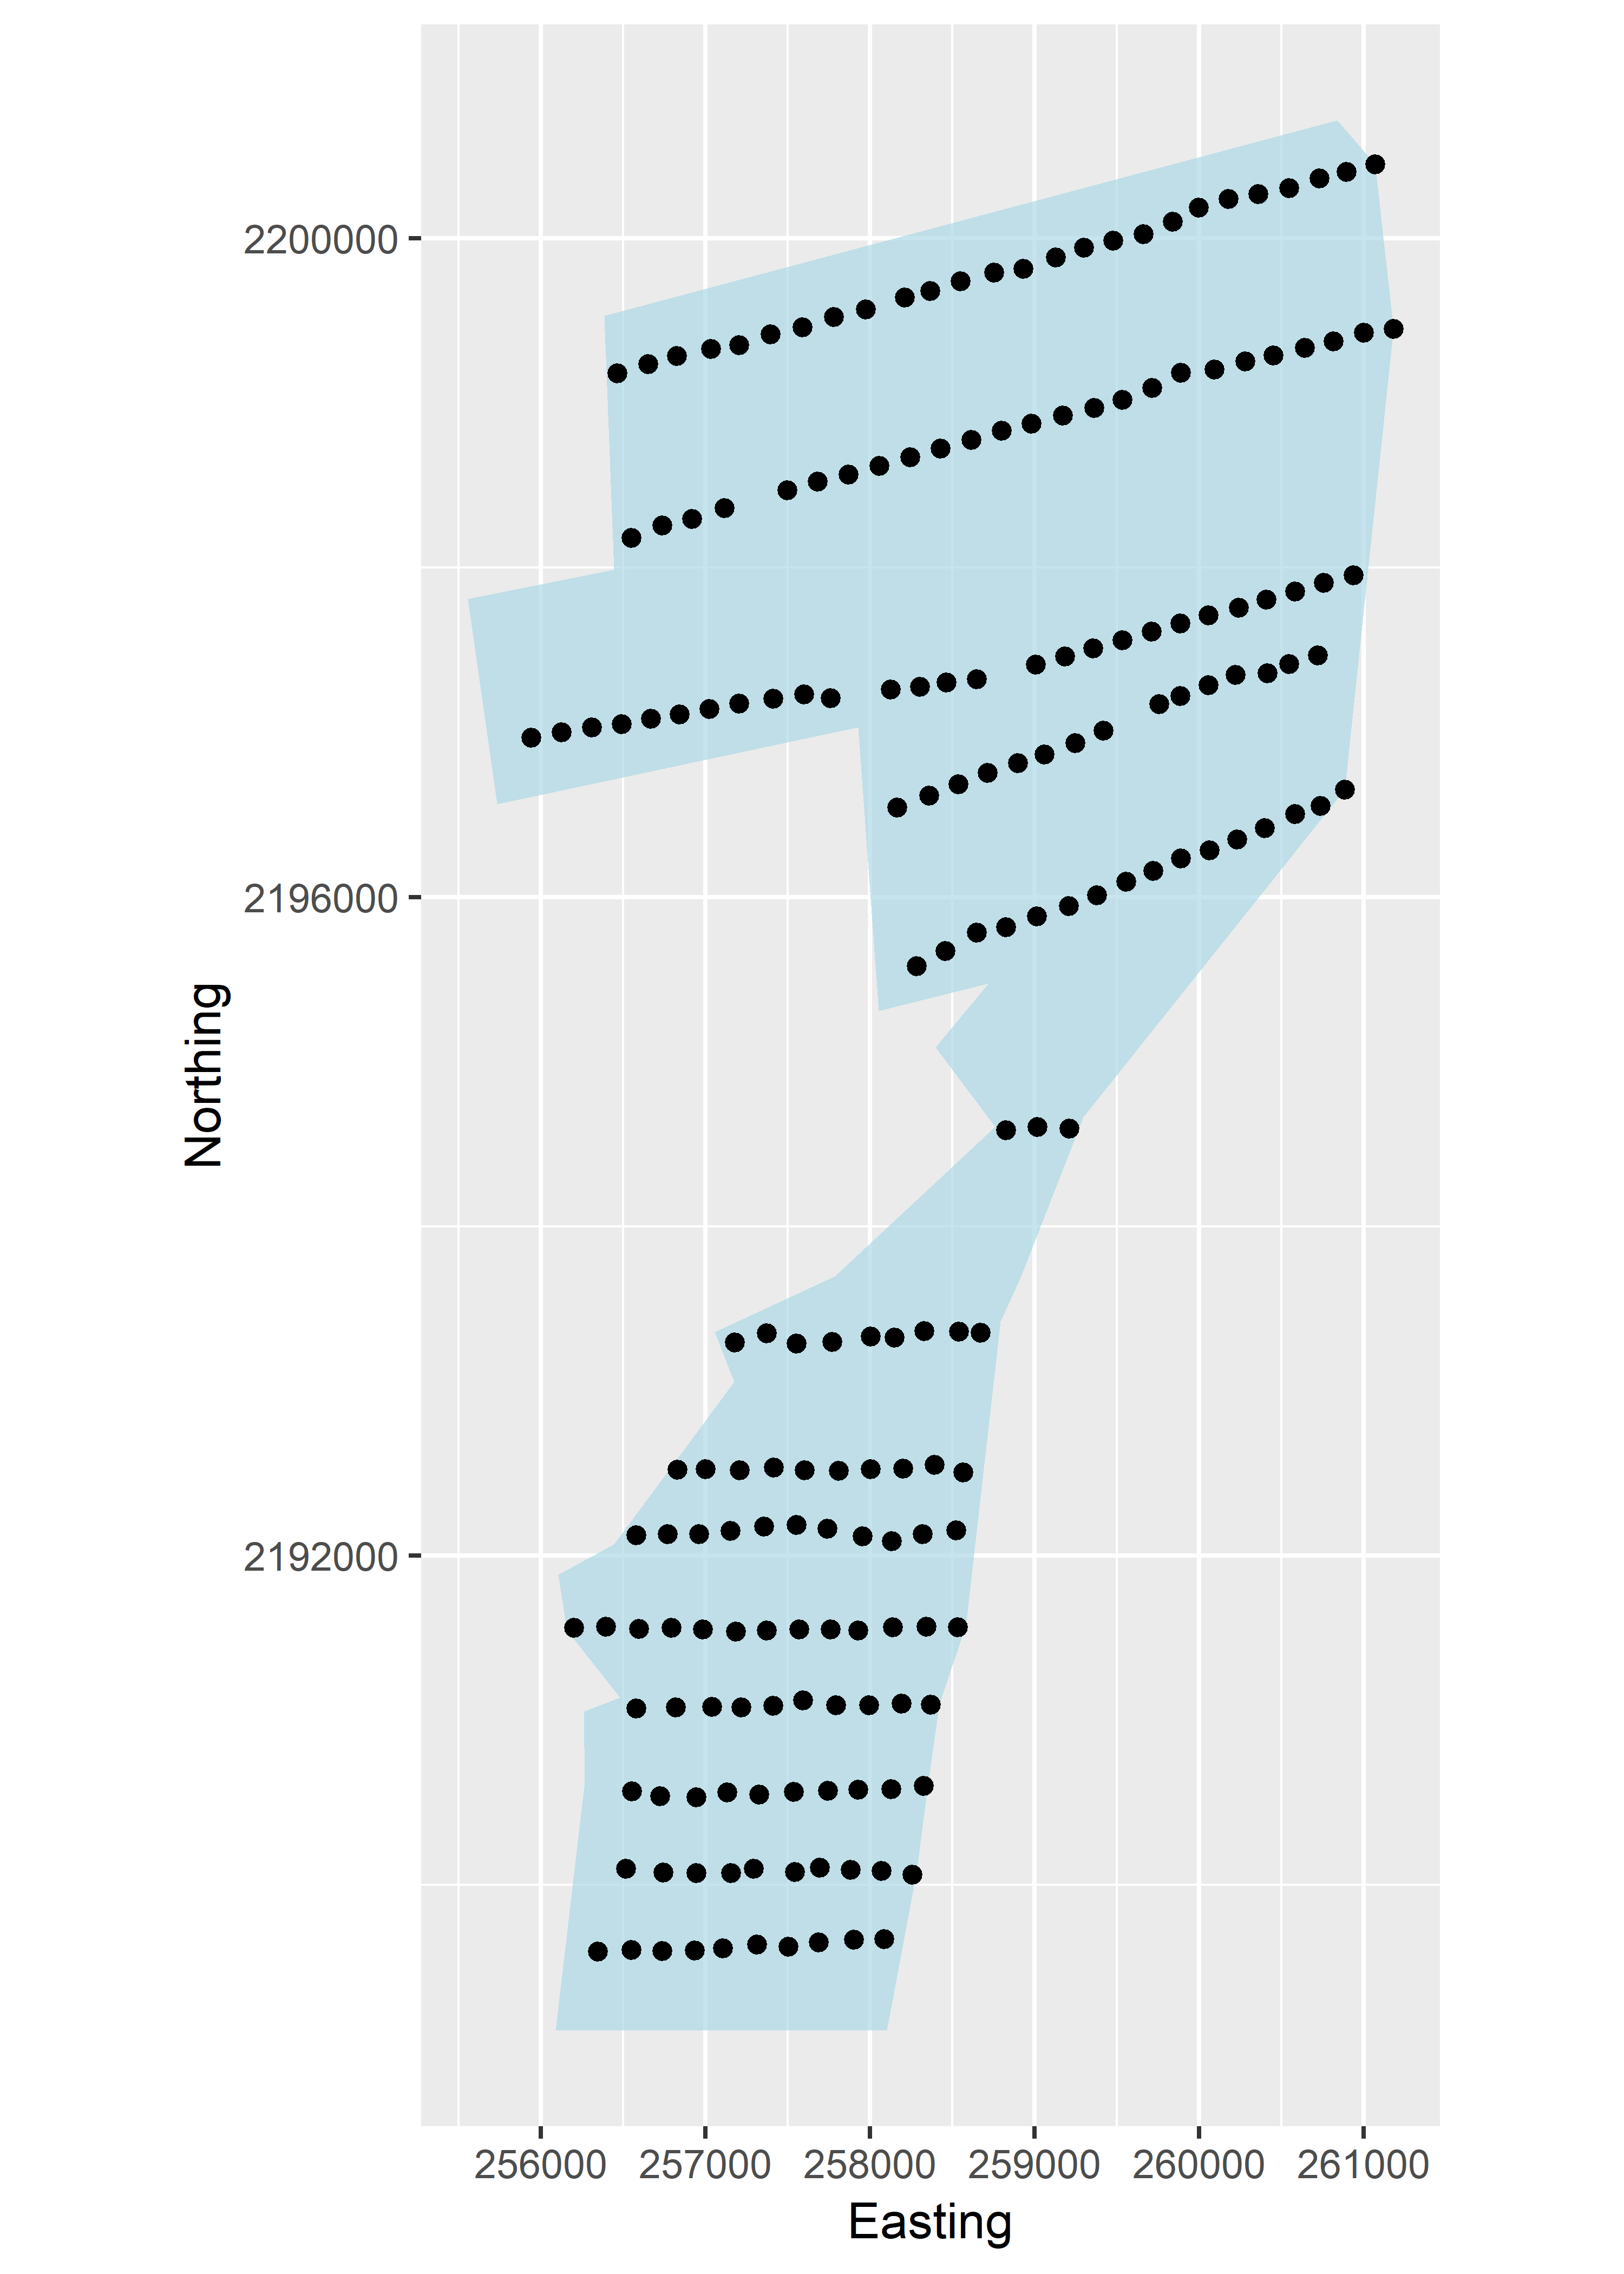
\includegraphics[scale=0.5]{figures/2002studyareapoints_pt}
	\caption{Study area (light blue) showing the 2002 survey points (black dots) in Hakalau Forest National Wildlife Refuge, \hawaii{} Island.}
	\label{fig:2002studyareapointspt}
\end{figure}

Surveys used point-transect methods, recording horizontal distances from survey points to individually detected birds. Surveys commenced at dawn and continued until 11:00 or halted when weather conditions exceeded prescribed conditions that hindered detecting birds (light rain, and wind and gust strength \textgreater Baufort scale 3). During 8-min counts trained observers recorded the species, exact distance to the nearest meter and detection type for each bird detected, along with the sampling conditions cloud cover, rain, wind strength, gust strength, and time of day each point was surveyed.   \cite{camp_population_2010,camp_statespace_2016} provide a detailed description of Hakalau, the open-forest study area and the bird surveys.

\subsection*{Data description}
[[ Need to update this with extended data ]]

For the purposes of our analysis we selected a single survey from the \akepa{} time series that contained on broad sampling of the study area with sufficient numbers of detections to estimate detectability. In 2002, 195 points were sampled using point-transect distance sampling methods within the 3,061 ha open-forest study area of Hakalau (Fig. \ref{fig:2002studyareapointspt}). On 67 points 152 \akepa{} were detected. The number of detections within each sampling unit ranged from zero to 6. 

%\begin{figure}
%	\centering
%	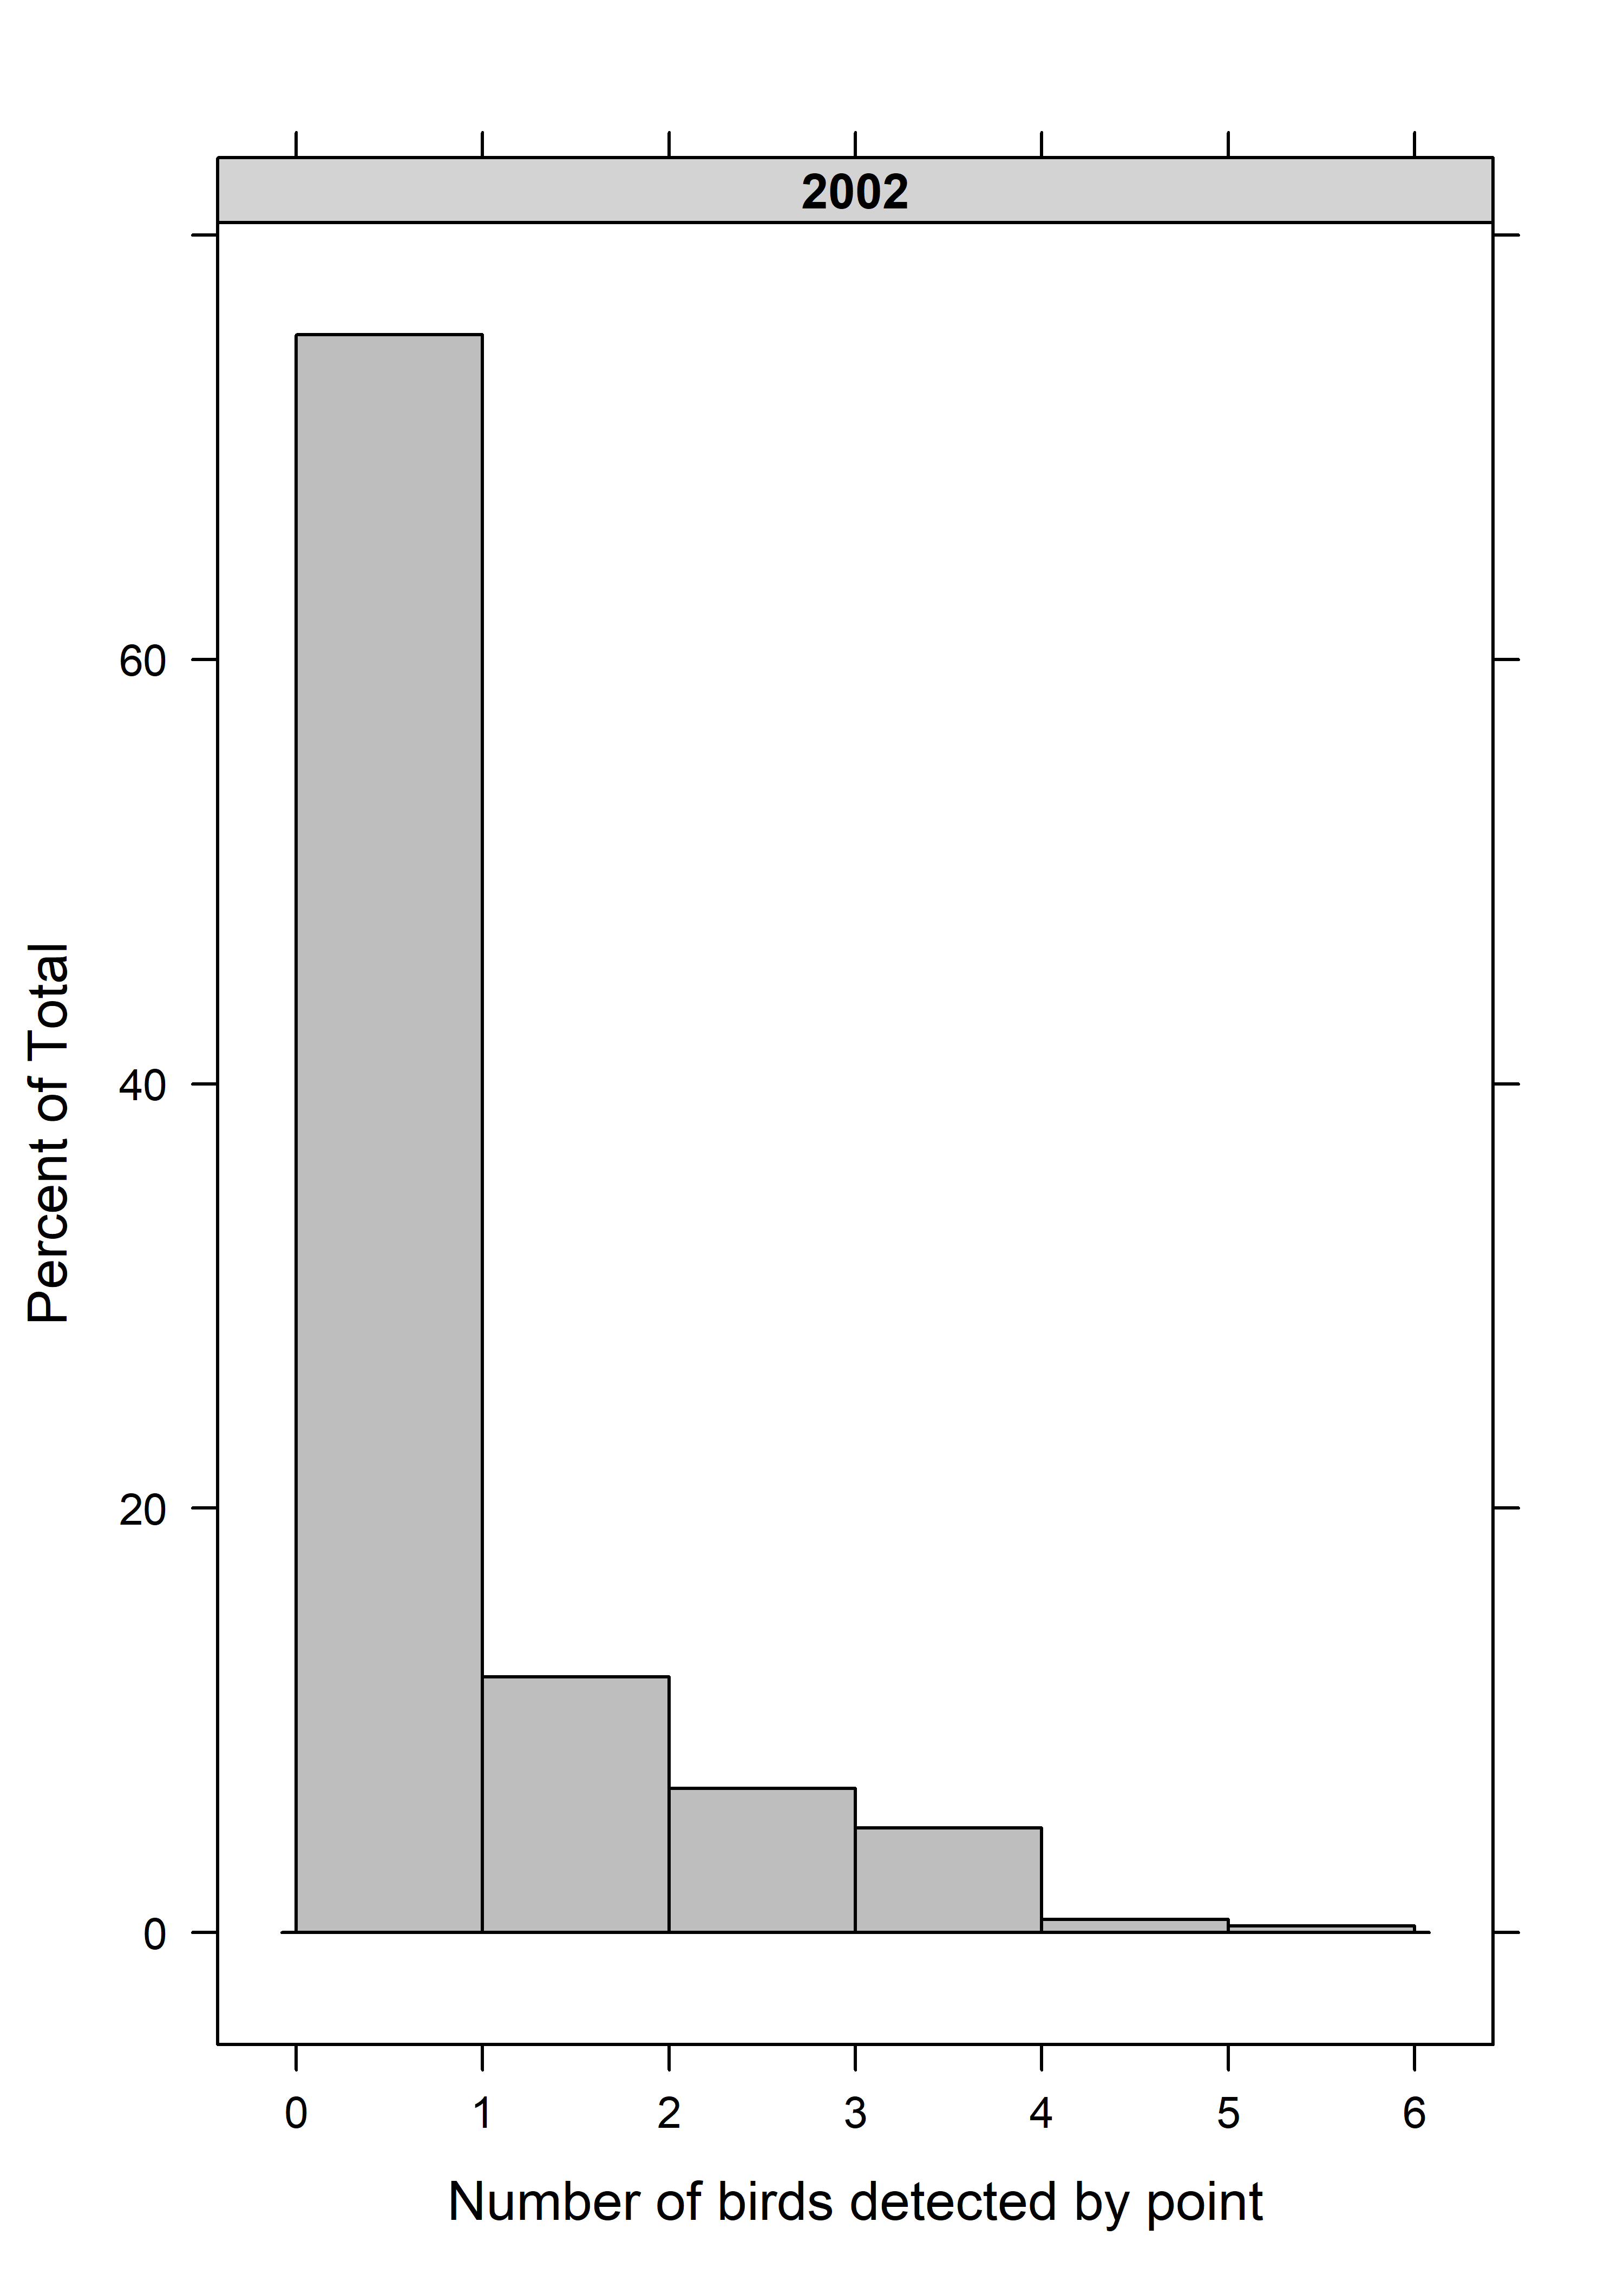
\includegraphics[scale=0.5]{figures/2002counts_pt}
%	\caption{Counts of \akepa{} by point during the 2002 survey.}
%	\label{fig:2002countspt}
%\end{figure}

% addtextend

\subsection*{Model specification in \texttt{inlabru}}


In this section we introduce \texttt{inlabru} syntax and provide example code to demonstrate how to specify the model.  First, we specify the SPDE model component as
\begin{lstlisting}
matern <- inla.spde2.pcmatern(mesh, 
                              prior.sigma = c(2, 0.01),    
                              prior.range = c(130, 0.01))
\end{lstlisting}
which uses penalised complexity priors for the hyperparameters of the GMRF \citep{simpson_penalising_2017}, setting $\mathbb{P}(\sigma > 2) = 0.01$ and $\mathbb{P}(\rho < 130) = 0.01$ where $\rho$ is the range of the Mat\'ern covariance.  The value of 130 was selected based on the minimum distance between sampling locations.     

Second, we specify the thinning probability function model component.  The data contains only distances from the observer so we use equation \eqref{intensity-incomplete} to specify the log thinning probability function as
\begin{lstlisting}
thinning_function <- function(distance, lsig){
    log(2*pi) + log(distance) + log_halfnormal(distance, lsig)
    }
\end{lstlisting}
where \texttt{log\_halfnormal} is the log half-normal detection function $\log g(r | \sigma) = -1/2(r/\sigma)^2$ and the argument \texttt{lsig} is $\log(\sigma)$.  The dataset contains a column named \texttt{distance} that contains the observed distances.  The software will search for the appropriate columns using the names of the arguments specified in this function.  To allow the software to distinguish between named covariates and parameters - which both appear as arguments of the function to be estimated - we must also specify a model components object
\begin{lstlisting}
cmp <- ~ Intercept + grf(map = coordinates, model = matern) + lsig 
\end{lstlisting} 
This object names all model components to be estimated.  Note that the \texttt{grf} component is a name we have chosen and not a function.  The software allows user-specified names for the \texttt{f()} function known to users of \texttt{R-INLA}. Note that \texttt{coordinates} is a keyword that allows users to supply their data in the form of a spatial object using the \texttt{sp} package \citep{pebesma_spatial_2005}.  

We can now specify the predictor formula using the components defined above.  
\begin{lstlisting}
fml <- coordinates + distance ~ Intercept + grf +
	thinning_function(distance, lsig)
\end{lstlisting}
To fit the model we specify starting values for the parameters, the domain of possible observed distances and fit the model using the \texttt{lgcp} function
\begin{lstlisting}
starting_values <- data.frame(grf = 0, lsig = 3.65, Intercept = 0)
W <- 60   # transect radius
distance_domain <- seq(.Machine$double.eps, W, length.out = 30)
lgcp(components = cmp, 
     data = obs,
     samplers = samplers,
     domain = list(distance = distance_domain),
     formula = fml,
     options = list(result = starting_values, max.iter = 30))
\end{lstlisting}
where our observed data is contained in a \texttt{SpatialPointsDataFrame} object named \texttt{obs}.  We also specify the \texttt{samplers} object, also a \texttt{SpatialPointsDataFrame}, which contains the locations of all sampling units.  Full scripts for the analysis are available in the supplementary materials.

\subsection*{Results}

The predicted mean of the posterior intensity is shown in \autoref{fig:intensity-mean-cv} along with a map of the coefficient of variation (CV) of the posterior intensity field on a regular prediction grid with cell area of approximately 1.7 hectares.  This shows a region of high intensity in the south and much lower intensity in the north, agreeing with a standard two-stage analysis of the same data (see Supplementary materials).  The CV plot shows that the CV in the posterior intensity field is lower areas with greater sampling effort.  There is clear preferential sampling and in the north estimated intensities are lower which also contributes to larger CV values.
\begin{figure}
	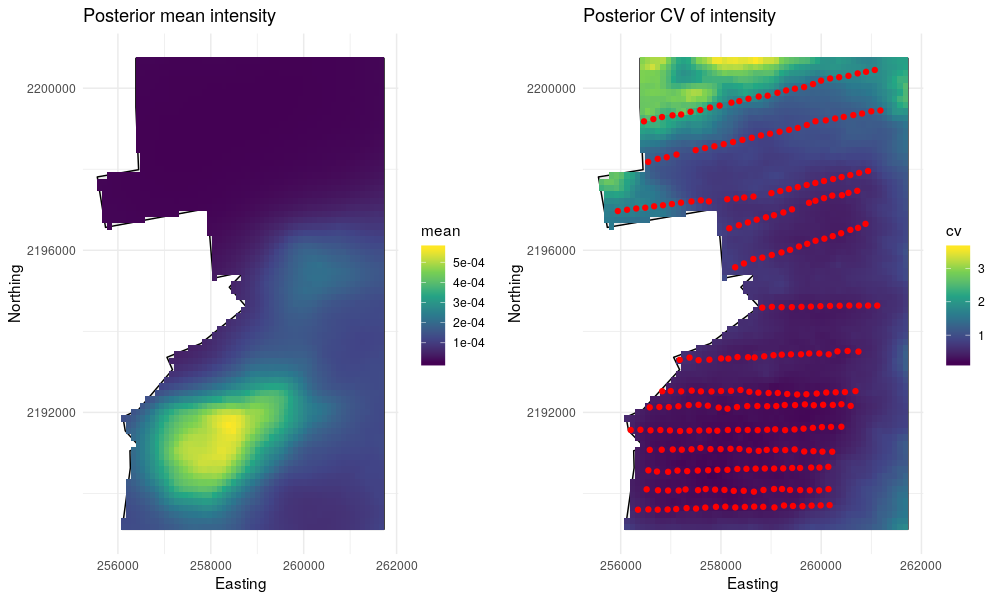
\includegraphics[scale=0.5]{figures/intensity_mean_cv.png}
	\caption{(left) Posterior mean of the intensity (right) Posterior coefficient of variation of the intensity}
	\label{fig:intensity-mean-cv}
\end{figure}

The fact that CV values are influenced both by sampling effort and the estimated intensity means other methods to visualise uncertainty in the posterior intensity field are also often considered. A common approach is to map the lower and upper quantiles corresponding to a 95\% credible interval for each prediction cell (\autoref{fig:intensity-quantiles}).
\begin{figure}
	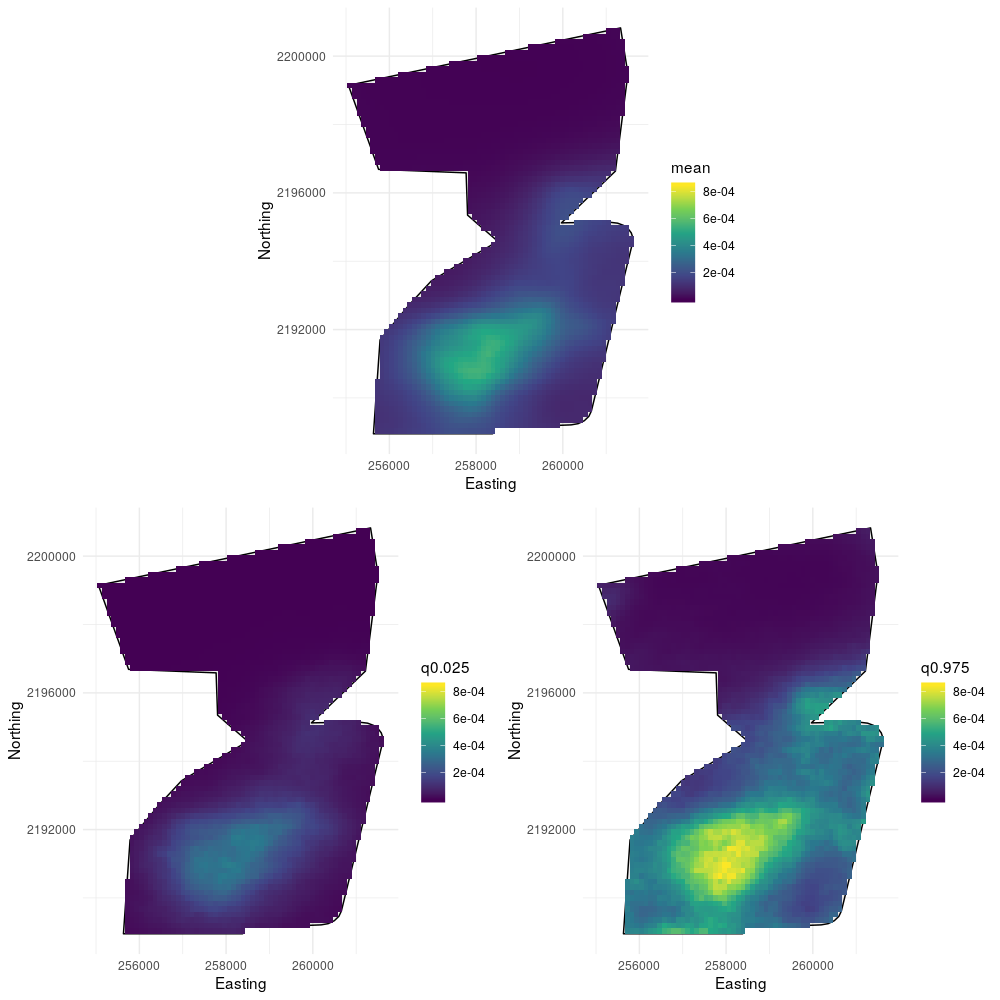
\includegraphics[scale=0.5]{figures/intensity_quantiles.png}
	\caption{The predicted posterior intensity summarised in three plots by the mean (upper),  0.025 quantile (lower left) and 0.975 quantile (lower right) for each prediction grid cell.  All three plots use a common colour scale}
	\label{fig:intensity-quantiles}
\end{figure}
Although commonly used, we believe quantile plots like those in \autoref{fig:intensity-quantiles} to be challenging to interpret and potentially misleading.  The temptation is to interpet these plots as showing possible intensity surfaces that produced the observed data.  Presenting these quantiles side by side in a single map obscures the problem of multiple hypothesis testing.  To demonstrate the fallacy of this we treated the lower and upper quantile plots as though they were intensities and integrated them to obtain an expected abundance estimate of approximately 3,300 for the 0.025 quantile and 12,400 for the 0.975 quantile.  A naive (and tempting) interpretation of these numbers is as upper and lower limits of the 95\% credible interval for abundance. However, these abundance estimates are outside the support of the posterior for abundance (see \autoref{fig:realized-abundance-posterior}).

As an alternative to the quantile maps we use excursion sets and excursion functions \citep{bolin_excursion_2015}.  This is a recent addition to the literature so we take some time here to define and elaborate on the concepts used.  This approach to representing variability in stochastic processes specifically considers the joint probability of events across multiple locations.  The positive excursion set with level $u$ for a function $f(s)$ with domain $\Omega$ is $A_u^{+}(f) = \{ s \in \Omega ; f(s) > u \}$ i.e. the set of all locations in $\Omega$ where $f$ exceeds the a threshold value $u$. For a stochastic process $\lambda(s)$ the positive excursion set with level $u$ and probability $1 - \alpha$ is
% Somehow keep this information somewhere in the paper:
%This difference between summaries of the posterior and possible intensity surfaces that are consistent with the data becomes clear if one generates realizations of the posterior intensity field.  Three such realizations are in \autoref{fig:intensity-realizations}.  There are some notable differences when compared to the mean and quantile summary maps.  Each realization has finer-grained spatial structure than the mean or quantile plots of the posterior intensity.  In practice, this indicates that we should expect more spatial structure in our collected data than what we might expect if we only look at the posterior mean of the field.  The summary plots hide the spatial structure the model has been able to estimate from the data.  In general, the mean of a random field will contain less spatial structure than realisations of the field.
%

\begin{equation*}
E_{u,\alpha}^{+}(\lambda) = \argmax_{D}\{\lvert D \rvert : \mathbb{P}\left[D \subset A_u^{+}(\lambda)\right] \geq 1 - \alpha \}
\end{equation*}
Note that $A_u^{+}(f)$ specifies a set for which a function $f(s)$ exceeds a threshold value $u$ for \textit{every location} in the set.  As such the positive excursion set $E_{u,\alpha}^{+}(\lambda)$ is the largest such set for which a threshold is exceeded simultaneously for all locations in the set.  Negative excursion sets can be similarly defined.  Excursion sets can be estimated by considering candidate sets for $D$ of increasing size and a sequential integration scheme to estimate probabilities.  An implementation is available in the \texttt{excursions} package \citep{bolin_calculating_2018} available through the Comprehensive R Archive Network \citep{r_2017}.

\autoref{fig:excursions} (left panel) shows the positive excursion set with a level corresponding to 1 bird per hectare with probability 0.95.  This figure can be interpreted in a natural way.  It is the largest region for which the intensity is greater than 1 bird per hectare for every location within the region, with probability 0.95.
\begin{figure}
	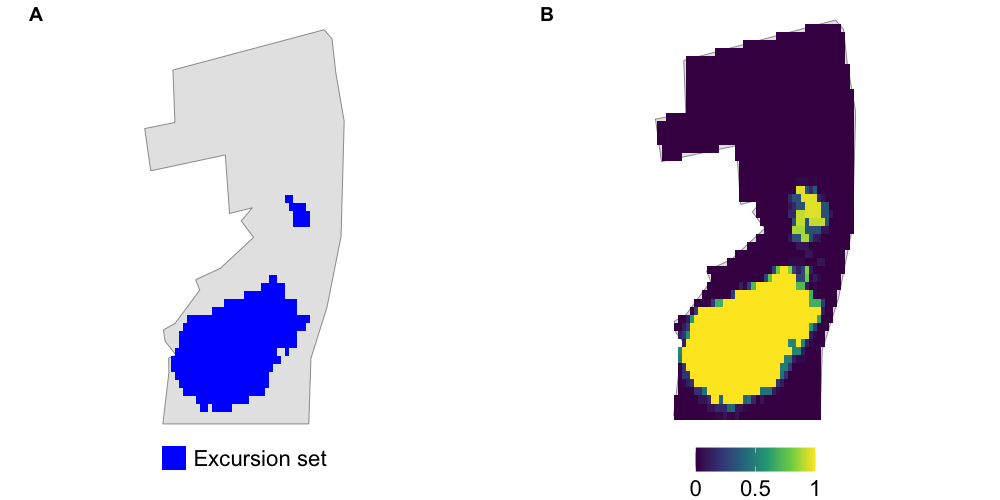
\includegraphics[scale=0.5]{figures/excursions.png}
	\caption{Left:  The positive excursion set with a level corresponding to 1 bird per hectare and probability 0.95.  Right: The positive excursion function with a level corresponding to 1 bird per hectare}
	\label{fig:excursions}
\end{figure}
To visualise multiple such maps we can use the excursion function $F_u^{+}(s) = \sup \{1 - \alpha ; s \in E_{u,\alpha}^+ \}$, which defines for each location something similar to a p-value.  For each $s$ it is the largest possible probability $1 -\alpha$ for which that location would be in the excursion set defined using probability $1 - \alpha$.  The excursion function with a level corresponding to 1 bird per hectare is shown in \autoref{fig:excursions} (right panel).  This figure can also be interpreted naturally.  It shows the largest possible probability for each location to be a member of a set in which the intensity exceeds a threshold simultaneously across all locations in the set. It is clear from the figure that regions on the edge of the excursion set would be included if the $\alpha$ value were allowed to increase slightly.  However, for regions in the north there is essentially no probability level for which those locations would be included in $A_u^{+}(\lambda)$.  In the above we used 1 bird per hectare as an illustrative threshold.  In applications multiple thresholds can be considered - based on the research question at hand.  An attractive feature of the excursions approach is that it forces researchers to identify values that are of interest and choose an acceptable probability of error given the wider context of the research.  

Given the issues of interpreting maps that simultaneously show summaries of the posterior random field it can often be informative to look directly at realisations themselves. Three such realizations are in \autoref{fig:intensity-realizations}.  
\begin{figure}
	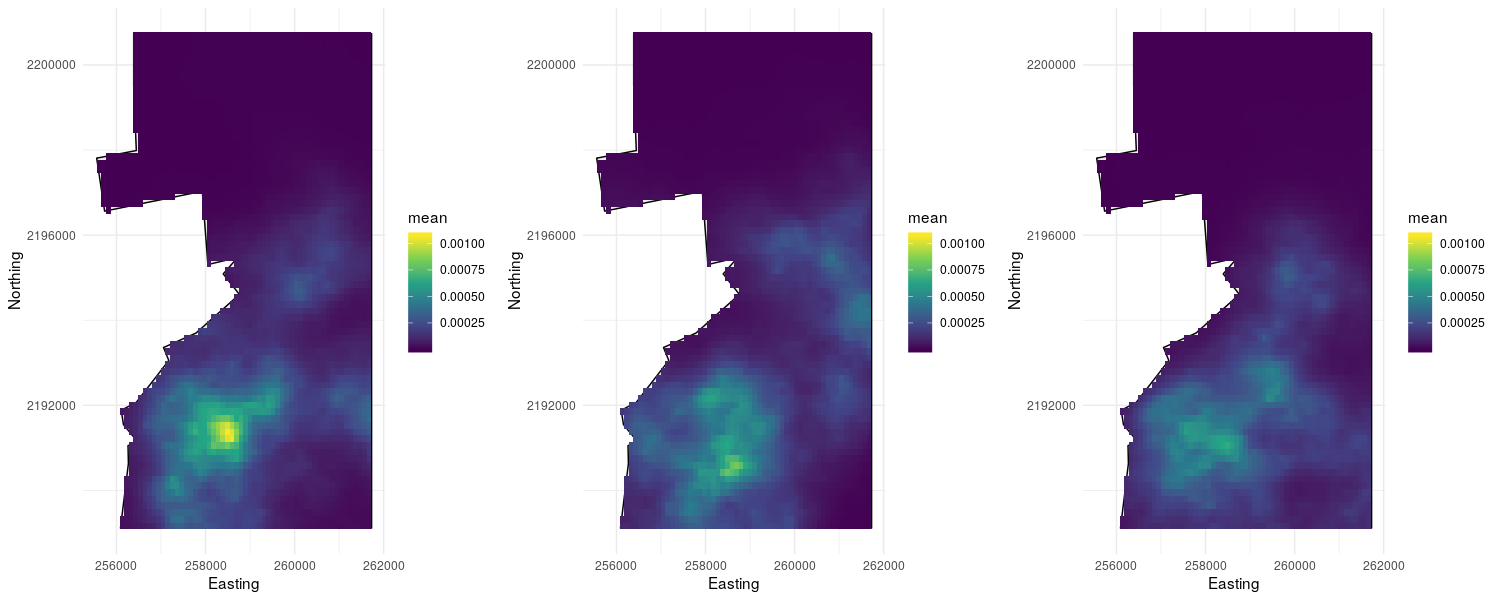
\includegraphics[scale=0.35]{figures/intensity_realized.png}
	\caption{Three realizations of the posterior intensity field}
	\label{fig:intensity-realizations}
\end{figure}
There are some notable differences when compared to the mean and quantile summary maps.  Note each realization has finer-grained spatial structure than the mean or quantile plots of the posterior intensity.  In practice, this indicates that we should expect more spatial structure in our collected data than what we might expect if we only considered the posterior mean of the field.  The summary maps hide the spatial structure the model has been able to estimate from the data.

Another key aim of performing distance sampling surveys is to estimate the abundance of the population of interest.  We describe here how to estimate the posterior for the abundance. Let $n$ denote the abundance of the population within the region of interest and $N = \int_{\Omega}\lambda(s)\mathrm{d}s$ its corresponding random variable within our Bayesian framework.  Integrating the mean of the posterior intensity field provides a point estimate for the abundance - the expected abundance.  We approximate the posterior $\pi(N | \lambda)$ by a monte-carlo method.  Taking $m$ monte-carlo samples  $\lambda_1, \ldots, \lambda_m$ of the posterior intensity field we estimate the posterior for the abundance as $\pi(N | \lambda) \approx 1 / m \sum_{i=1}^m \pi (N | \lambda = \lambda_i)$. Each $\pi(N | \lambda = \lambda_i)$ is a Poisson probability mass function with rate parameter $\int_{\Omega}\lambda_i(s)\mathrm{d}s$. \autoref{fig:realized-abundance-posterior} shows the approximate posterior for $N$ with $m = 20,000$.  This allows us to estimate the probability for any specific value of realised abundance $n$ by calculating $\pi(N = n | \lambda)$.  For reference, \autoref{fig:realized-abundance-comparison} shows a single Poisson PMF with rate parameter equal to the expected abundance.
\begin{figure}
	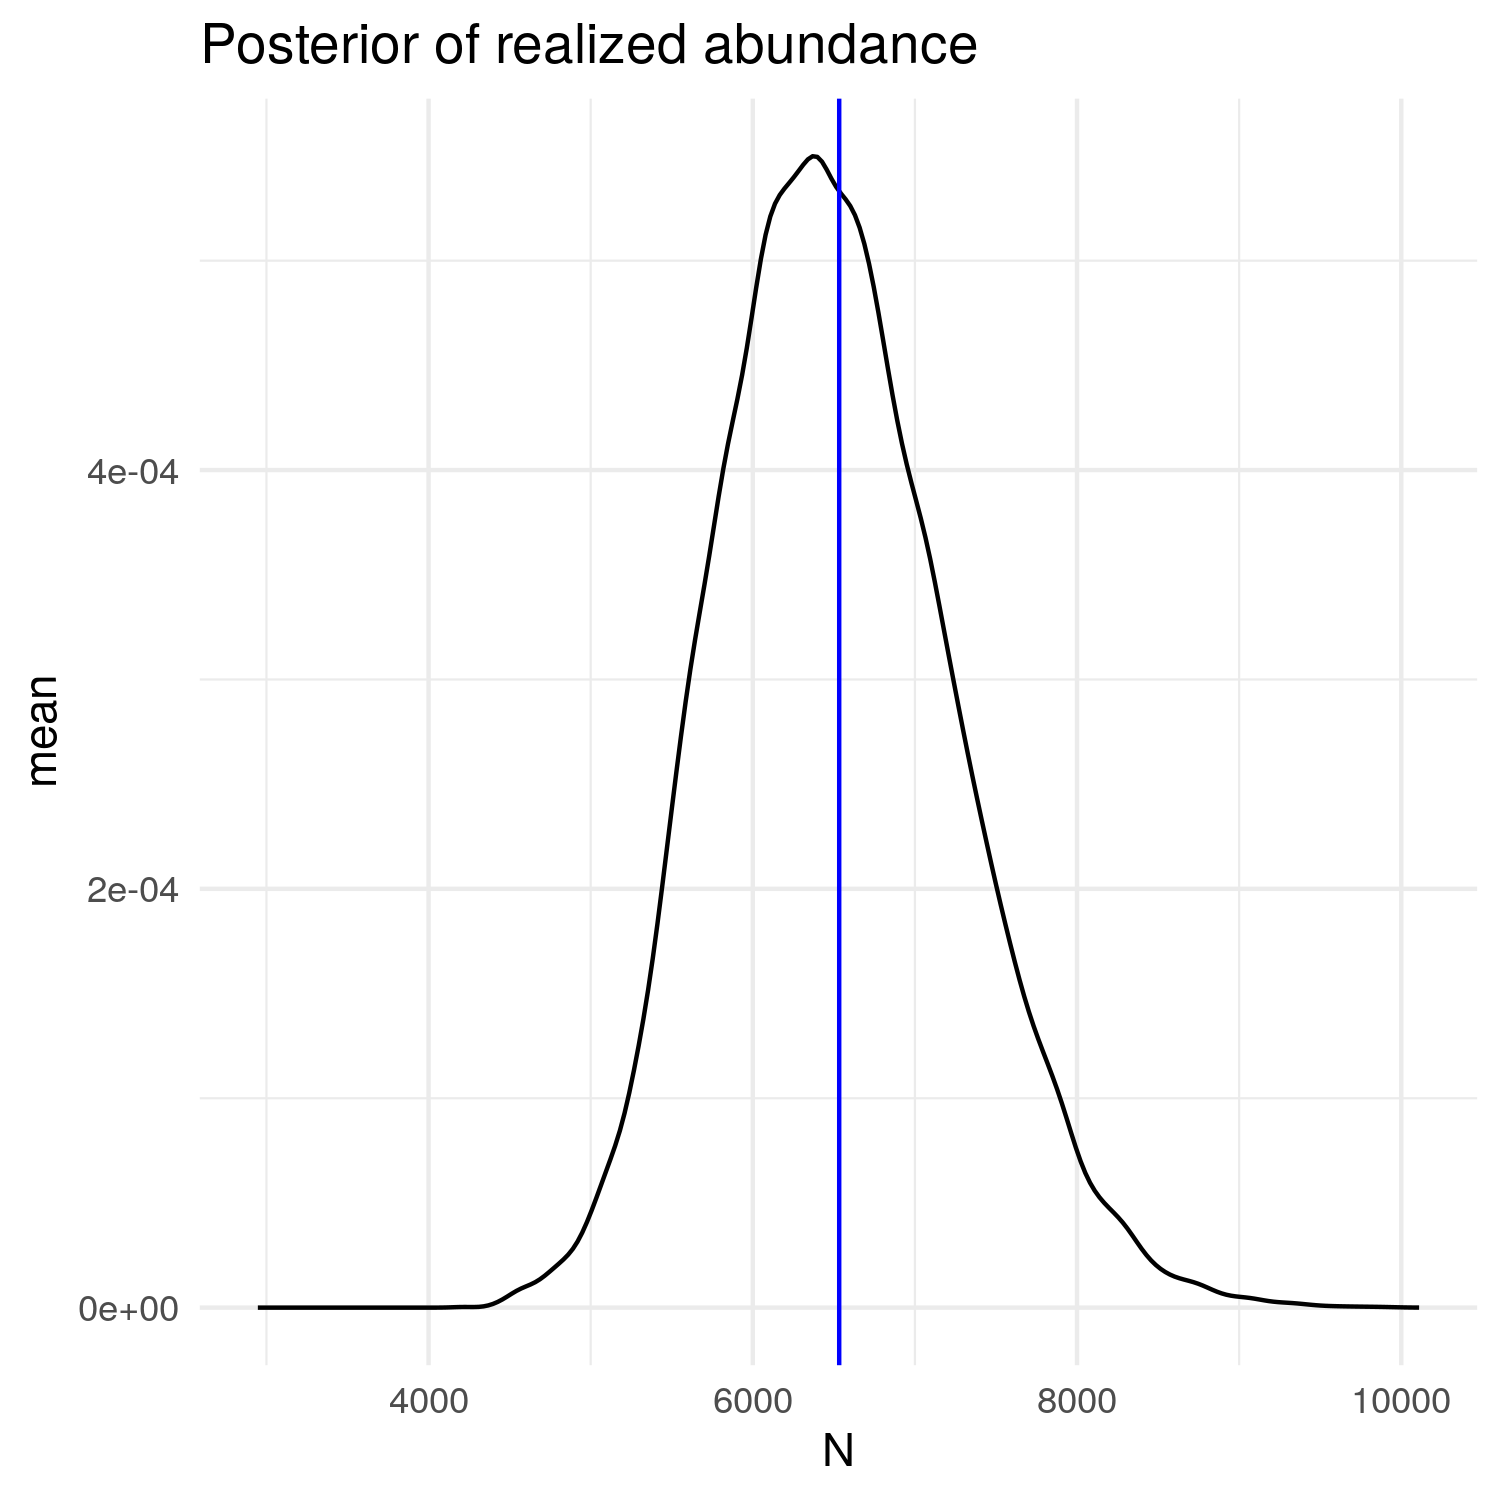
\includegraphics[scale=0.6]{figures/realized_abundance_posterior.png}
	\caption{Posterior of realized abundance.  The blue line marks the expected abundance}
	\label{fig:realized-abundance-posterior}
\end{figure}
\begin{figure}
	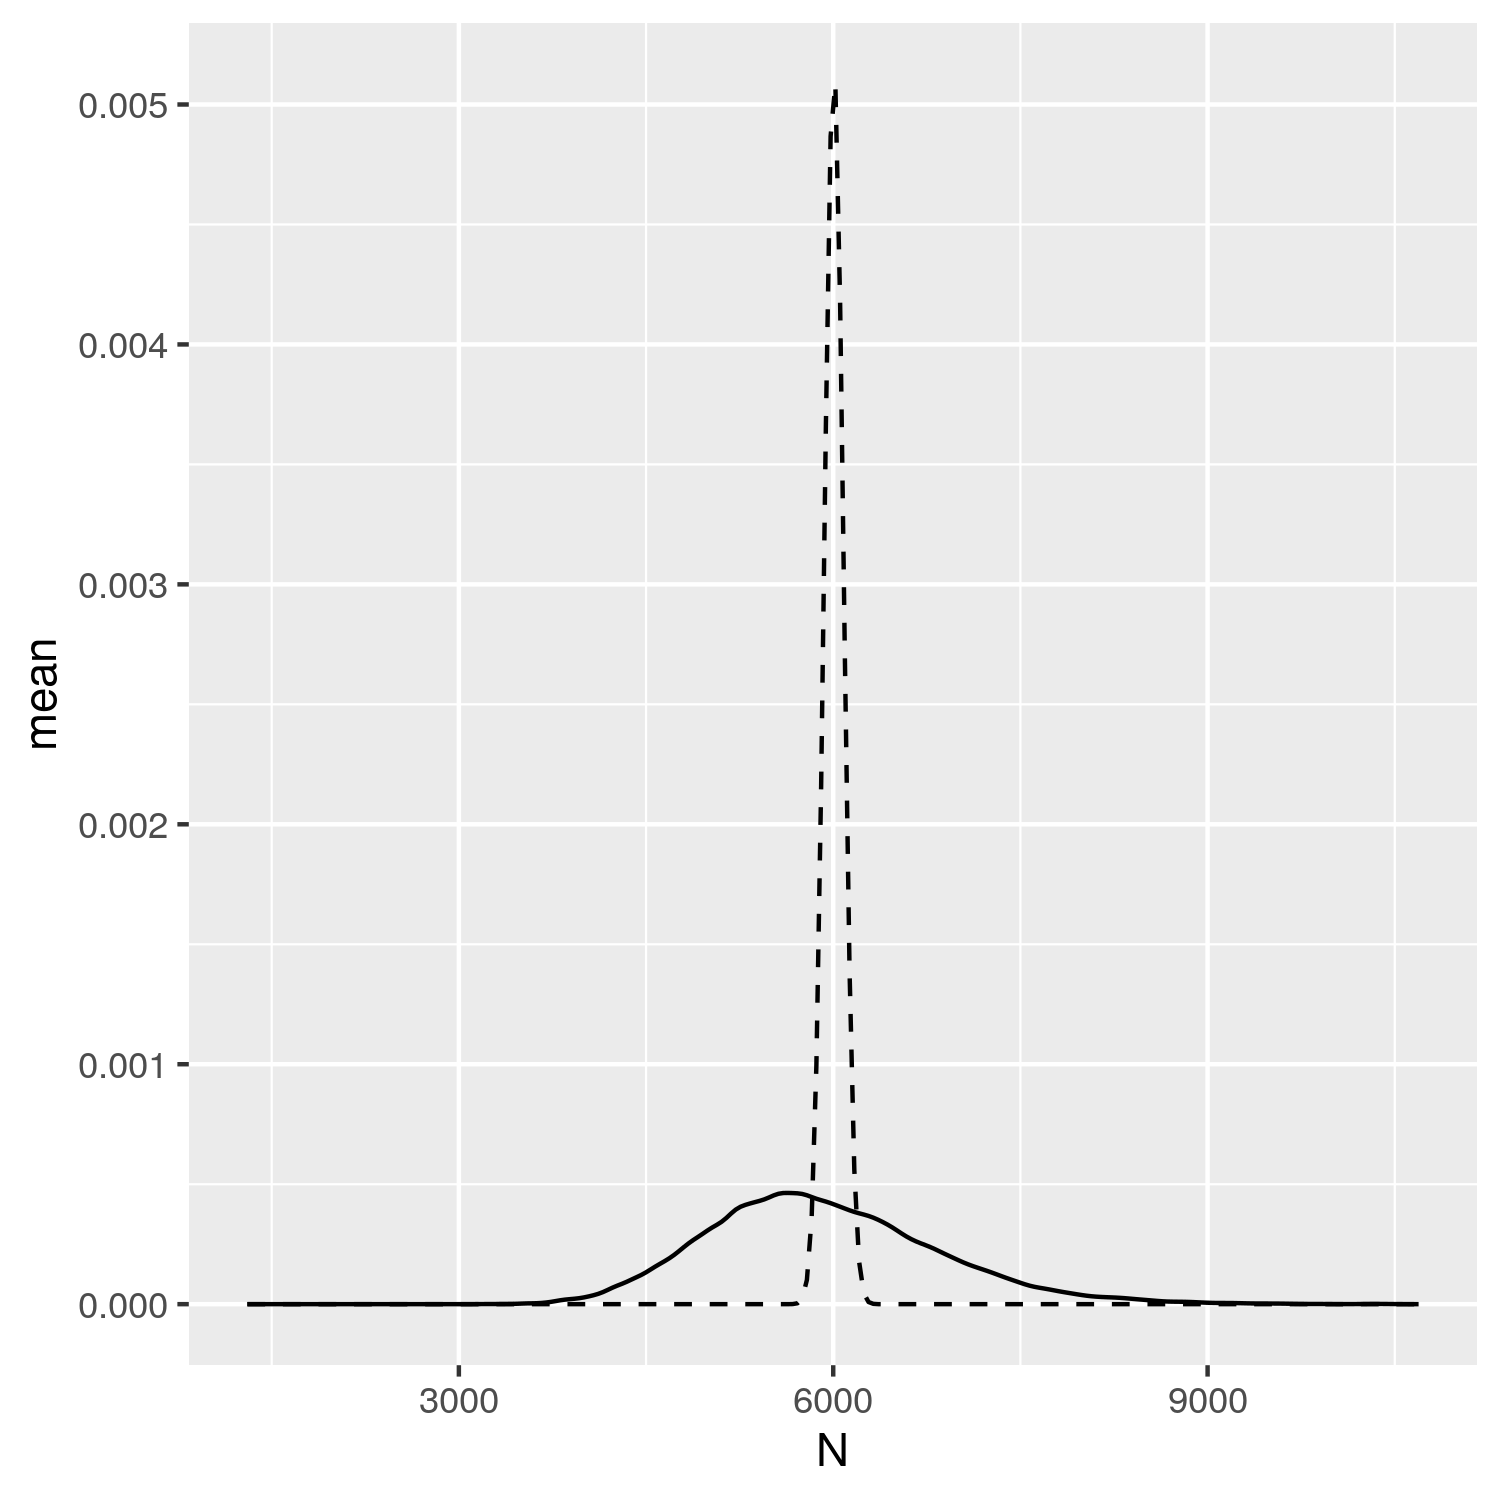
\includegraphics[scale=0.6]{figures/realized_abundance_vs_exp.png}
	\caption{Solid:  Posterior of realized abundance.  Dashed:  Poisson PMF with rate parameter $\mathbb{E}[\Lambda]$}
	\label{fig:realized-abundance-comparison}
\end{figure}
We note here that in a GAM approach it is common to only report the estimated expected abundance and the uncertainty in this estimate.  This does not include the additional variability that comes from the Poisson distribution with a rate parameter equal to the expected abundance.  

Finally, we show that the one-stage model has estimated a plausible detection function.  \autoref{fig:half-normal} shows a summary of the posterior for the detection function, plotting the posterior mean along with 95\% credible intervals.  We note again that all model summaries shown in this section are based on monte-carlo sampling of the joint posterior of all model parameters.  As such all the plots incorporate the uncertainty in the detection process.  
\begin{figure}
	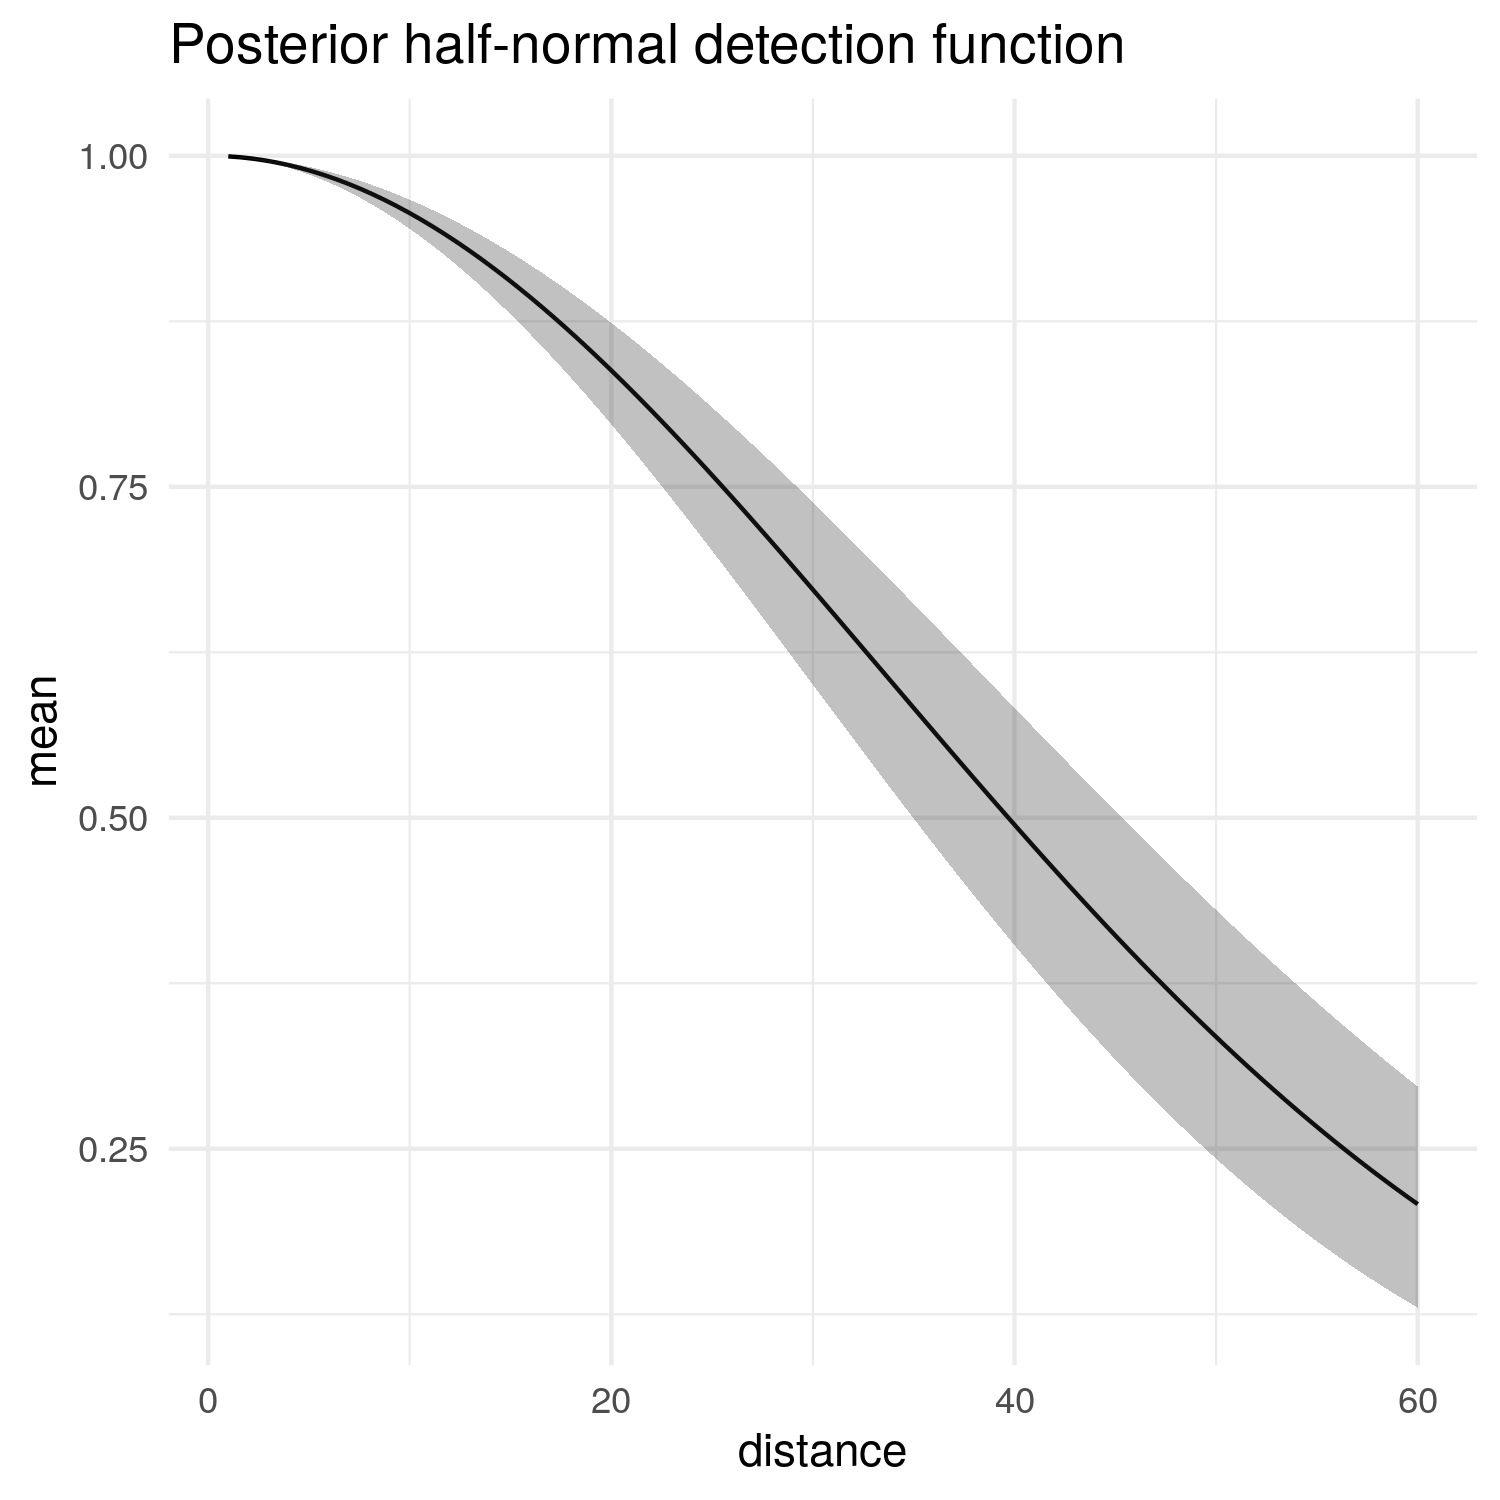
\includegraphics[scale=0.6]{figures/halfnormal.png}
	\caption{Posterior detection function}
	\label{fig:half-normal}
\end{figure}

\bigskip

\newpage

\section*{Discussion}

\subsection*{General remarks}

The most common method to analyse distance sampling data is a two-stage approach with a generalised additive model that includes a spatial smoothing spline.  The approach here of specifying a point process model and including an SPDE effect can seem fundamentally different.  However, these two approaches are related and an analysis of the \akepa{} data using the GAM approach provides similar point estimates.  There is a correspondence between SPDEs and smoothing splines: the smoothing spline is an estimator of the posterior mean of the SPDE \citep{kimeldorf_spline_2002}.  The SPDE and the smoothing spline play a similar role within the model and the resulting mean field map looks similar in both approaches.  
In addition, it can appear as though the point process model avoids the need to bin data into counts and so avoids some loss of information. This is not the case since we also applied the standard distance sampling assumption of constant intensity within each point transect.  This can be thought of as the point process version of binning data into counts since the location of points within transects does not inform the spatial distribution of points across the whole study region.  The main advantage of the log-Gaussian Cox process is that the discretisation of space occurs during the step of approximating the GRF.  This is in contrast to motivating the discretisation by the act of binning the data into counts so as to create a response variable that can be analysed using a GAM model.  We also note that \texttt{inlabru} provides functionality for fitting models with multiple likelihoods \citep{bachl_inlabru_2019}.  As such our approach is extendible to more complicated contexts such as marked point processes.    

We believe the excursions approach is a valuable addition to the literature on communicating uncertainty in estimated surfaces.  For species distribution modelling this has the potential to be a useful tool for model evaluation and communication with stakeholders.  In particular the approach requires users to decide (i) a threshold or set of threshold values of interest and (ii) an acceptable probability of error. 
We believe that, in most situations, these decisions should be made by domain experts who have an understanding of the phenomena of interest, the set of possible decisions that may be taken on the basis of the analysis and the consequences of error.  Once these decisions have been made the statistician can then proceed accordingly, providing outputs  that inform on quantities of interest with a level of uncertainty that stakeholders have agreed is acceptable.  We note that the excursions approach applied here has the potential to be useful in other methods of species distribution mapping, environmental statistics and spatial statistics in general.  There is the potential to use excursions to motivate both the \textit{definition} and \textit{estimation} of concepts of interest to ecologists, such as a species' home range or the notion of occupancy. 

\subsection*{Possible future research}

Here we applied the iterated INLA approach in order to estimate the half-normal detection function which is non-linear in its $\log \sigma$ parameter.  We note that this approach provides a general framework for estimating parametric functions from data and is not restricted to detection functions in a distance sampling model.  The \texttt{inlabru} software allows users to specify the model in an intuive and modular way.  Users write individual functions to define (possibly non-linear) model components and specify how these are combined to form the additive predictor.  By additive we mean a predictor that is a sum of model components, and not necessarily additive in terms of parameters to be estimated.

We presented a simple choice for the detection model.  The half-normal function has only one parameter to be estimated but other, more flexible, detection functions are common in applications.  The potential to include further flexibility in the detection model through covariates or random-effects is an open research question and would dramatically increase the usability of our approach presented here. Increasing the number of parameters to estimate in the non-linear model components may run into computational challenges.  This has yet to be explored.  

Model selection is a general challenge for models with spatially structured random effects.  Traditional tools of model assessment and selection do not apply in many contexts.  For model assessment we advise a pragmatic approach based on comparing summaries of posterior samples to the observed data. A moodel selection procedure is useful to users to justify decisions regarding which covariates to include, whether or not to include a spatially structured random effect, and if so, what type of effect should be used. 

\bibliographystyle{chicago}
\bibliography{paper}

\end{document}
